\chapter*{Vorwort}
\label{cha:Vorwort}
\addcontentsline{toc}{chapter}{\nameref{cha:Vorwort}}

Im Jahr 2017 wurden mehr als 1,8 Milliarden browser-fähige Endgeräte weltweit verkauft. Der technologische Fortschritt in Hardware und Software erlauben es dieser großen Masse an Zugängen zum Internet eine große Vielfalt an Applikationen nahezu überall zu nutzen. Seien es Business-, Unterhaltungs-Applikationen, oder Spiele jeglicher Art.\\
Dem gegenüber steht ein immer noch riesiger Markt für Retro-Spiele und Handhelden, die dem Drang nach mehr Grafikdetails und Leistungshunger aus dem Weg gehen und durch Charme mit Pixeln und Kindheitserinnerungen punkten. Spiele-Klassiker wie PacMan, Tetris, Mario und \uvm sind auch heute noch auf jedem Handhelden zu finden. Es gibt weiterhin Absatz auch für alte Plattformen wie die Atari, oder den C64. Wer den C64 und Spiele in einem Satz nennt muss auch eines der meistverkauften Spiele für den als "Brotkasten" bekannten Computer nennen: \emph{Archon}.\\
\index{Archon!Cover}
\begin{figure}[htp]
\centering
\captionsetup{justification=centering}
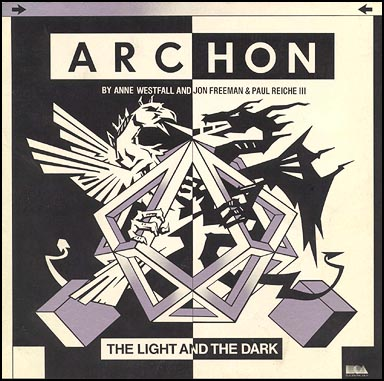
\includegraphics[width=0.50\textwidth]{Archon.jpg}
\caption[Archon - Cover]{Archon - Cover\footnotemark}
\label{fig:Archon_Cover}
\end{figure}
\footnotetext{\Quelle{C64-Wiki, \url{https://www.c64-wiki.com/wiki/Archon}}}



Der Schwerpunkt dieser Arbeit befasst sich mit der Umsetzung des bekannten Retro-Spiels Archon mit Web- und 3D-Technologien


Die klaren Vorteile des Web als Plattform, auch für Spiele, sind die Offenheit, der einfache Zugang und die immer weiter steigende Unterstützung neuer Technologien.\\
Sogenannte Spiele-Engines, also Bibliotheken die sich um die meisten, generellen Problemstellungen eines Spiels und seiner Entwicklung kümmern, gibt es daher allerlei.
So sind heutzutage hardwarebeschleunigte 3D-Visualisierung und Echtzeitkommunikation im Webbrowser Stand der Technik.
In dieser Arbeit soll die Verschmelzung von State of the Art Webtechnologien mit einem Retro-Spiel erfolgen.\\
"Archon" genoss für Atari und C64 großen Erfolg, ähnlich vieler anderer Spiele für die Konsolen der 80er.
\todo{Anmerkung \& Recherche zu Erfolg von Archon belegen!}
Das Spiel dient daher als sehr gutes Exempel für die Möglichkeiten des Webs als Spieleplattform, aber auch der Möglichkeiten und Freiheiten des Webs für jede andere Art von Applikation.